%%%%%%%%%%%%%%%%%%%%%%%%%%%%%%%%%%%%%%%%%
% Programming/Coding Assignment
% LaTeX Template
%
% This template has been downloaded from:
% http://www.latextemplates.com
%
% Original author:
% Ted Pavlic (http://www.tedpavlic.com)
%
%%%%%%%%%%%%%%%%%%%%%%%%%%%%%%%%%%%%%%%%%

%----------------------------------------------------------------------------------------
%	PACKAGES AND OTHER DOCUMENT CONFIGURATIONS
%----------------------------------------------------------------------------------------

\documentclass{article}

\usepackage[utf8]{inputenc} %unix-windows-compatible
\usepackage{commath}
\usepackage{fancyhdr} % Required for custom headers
\usepackage{lastpage} % Required to determine the last page for the footer
\usepackage{extramarks} % Required for headers and footers
%\usepackage[usenames,dvipsnames]{color} % Required for custom colors
\usepackage{graphicx} % Required to insert images
\usepackage{listings} % Required for insertion of code
\usepackage[section]{placeins}
\usepackage{caption} % to set figure captions in minipage
\usepackage{amsmath}
\usepackage{amssymb}
\usepackage{amsthm}
\usepackage{tikz}
\usepackage{algorithm}
\newcommand{\pushcode}[1][1]{\hskip\dimexpr#1\algorithmicindent\relax}
\usepackage[noend]{algpseudocode}

% Set up the header and footer
\pagestyle{fancy}

%\setlength\parindent{0pt} % Removes all indentation from paragraphs
\renewcommand\thesubsection{\thesection.\alph{subsection}}
\newcommand*\tageq{\refstepcounter{equation}\tag{\theequation}}


\newtheorem{mydef}{Definition}
\newtheorem{theo}{Theorem}
\newtheorem{cor}{Corollary}
%----------------------------------------------------------------------------------------
%	CODE INCLUSION CONFIGURATION
%----------------------------------------------------------------------------------------
% Default fixed font does not support bold face
\DeclareFixedFont{\ttb}{T1}{txtt}{bx}{n}{12} % for bold
\DeclareFixedFont{\ttm}{T1}{txtt}{m}{n}{12}  % for normal

\usepackage{color}
\definecolor{deepblue}{rgb}{0,0,0.5}
\definecolor{deepred}{rgb}{0.6,0,0}
\definecolor{deepgreen}{rgb}{0,0.5,0}
\lstset{language=Python, 
breaklines=true, 
tabsize=4,
basicstyle=\ttm,
otherkeywords={self},            
keywordstyle=\ttb\color{deepblue},
emph={MyClass,__init__},         
emphstyle=\ttb\color{deepred},   
stringstyle=\color{deepgreen},
frame=tb,                        
showstringspaces=false            
}% 
%\setcounter{secnumdepth}{0} % Removes default section numbers

%----------------------------------------------------------------------------------------
%	NAME AND CLASS SECTION
%----------------------------------------------------------------------------------------

\newcommand{\Title}{Enhanced exact algorithms for discrete bilevel linear
	problems} % Assignment title
\newcommand{\Seminar}{Seminar: Selected Topics in bilevel optimization} % Course/class
\newcommand{\Author}{Leon Eifler}
\newcommand{\fett}[1]{\mathbf #1}
\newcommand{\Real}{\mathbb{R}}
% Your name
%\newcommand{\ID}{327468} % Your name

\title{
	\centering
	\begin{figure*}[!hb]
		\begin{minipage}{1\textwidth}
			\hspace*{-.06\linewidth}
		\end{minipage} 
	\end{figure*}
	\vspace{5cm}
	{\huge\textbf{\Title}}\\ 
	\vspace{1cm}
	{\huge{\Seminar}\\}
	\vspace{0.6cm} 
	{\mdseries\large \Author }
	\vspace{1cm}
}


%----------------------------------------------------------------------------------------

\begin{document}
	
	\maketitle
	\newpage
%----------------------------------------------------------------------------------------
%	TABLE OF CONTENTS
%----------------------------------------------------------------------------------------
\section{Overview}

We present the work of Caramia and Mari \cite{Caramia2015}, who introduced two new exact algorithms for solving bilevel linear problems in which all the variables are discrete. These Discrete Bilevel Linear Problems (DBLPs) can be defined as:

		\begin{alignat*}{2}
		\text{(DBLP)} \quad \min_{x,y} F(x,y) &= c_1^Tx +c_2^Ty&& \\
		\text{s.t.} \quad &Cx + Dy \le e&& \\
		&x \in \mathbb{Z}^n_+ \\
		&y \in \arg \min_y&& f(y) = d^T y \\
		&\text{s.t.} &&Ax+By \le b \\
		& &&y \in \mathbb{Z}^m_+
		\end{alignat*}
		
The first Algorithm is a cutting plane method, where each added inequality separates multiple bilevel infeasible solutions. The second is a branch and cut method that exploits a geometric property of bilevel linear problems. 
The computational results are compared to the method proposed by DeNegre and Ralphs \cite{DeNegre2009}.

\section{Preliminaries}

We will introduce notation that we will need when discussing feasible solutions of (DBLP). 
First we define the \textit{constrained region}, where we omit integrality requirements on the variables.
\begin{equation*}
	S = \{(x,y) \ | \ x \in \mathbb{Z}^m_+, y \in \mathbb{Z}^m_+, Cx+Dy \le e, Ax + By \le b \}
\end{equation*}
For each possible value of the leader variables $x$ we define the \textit{followers feasible set}
\begin{equation*}
	\Omega_y(x) = \{y \ | \ y \in \mathbb{Z}^m_+, By \le b - Ax \}
\end{equation*}
and the set of all $y$ that minimize the followers objective, called the \textit{reaction set}
\begin{equation*}
	R_y(x) = \arg \min_y \{f(y) \ \text{s.t. } y \in \Omega_y(x).
\end{equation*}
Finally the set of all bilevel feasible solutions, the \textit{inducible region}, is defined as
\begin{equation*}
	IR = \{(x,y) \ | \ x \in \mathbb{Z}^n_+, Cx+Dy \le e, y \in R_y(x)\}.
\end{equation*}
The relaxation that we will use to solve (DBLP) we call the Single Level linear Problem (SLP), defined as
\begin{align*}
\text{(SLP)} \quad &\min_{x,y} F(x,y) = c_1^Tx +c_2^Ty \\
&\text{s.t.} \quad (x,y) \in S.
\end{align*} 
Note that this is indeed a relaxation as every optimal solution of (SLP) is a lower bound to the optimal solution of (DBLP).

\section{A cutting plane method}
\label{cp}

The basic idea of the cutting plane method can be described as follows
\begin{description}
	\item[Solve relaxation] Solve (SLP) and obtain an optimal solution $(\bar x, \bar y)$.
	If it is bilevel feasible, then (DBLP) is solved.
	\item[Add inequality] If $(\bar x, \bar y)$ is not bilevel feasible, add an inequality to (SLP) that cuts off all bilevel infeasible solutions at $\bar x$. Then solve the new relaxation again and repeat until (DBLP) is solved.
\end{description}

We will now give a detailed explanation of this inequality. Let $(\bar x, \bar y)$ be an optimal solution of (SLP) that is not bilevel feasible. Then there exists a bilevel feasible point $(\bar x, \hat y)$ such that $f(\hat y) < f(\bar y)$. Now we introduce a valid inequality that is only active at $x = \bar x$ 
\begin{equation*}
		f(y) \le f(\hat y) + L \|x-\bar x\|_{\infty}.
\end{equation*}
This non-linear inequality can be reformulated as an optimization problem 
\begin{align*}
f(y) \le f(\hat y) + L \hat z, 
\end{align*}
where $\hat z$ is the optimal solution of 
\begin{align*}
(P_{\hat z}) \quad \min_{z} z \\
\text{s.t.} \quad z &\ge x_i - \bar x_i \quad i = 1,\dots,n \\
z &\ge \bar x_i - x_i \quad i = 1,\dots,n.
\end{align*}
Adding this to (SLP) turns it into a bilevel problem itself, but with continuous follower variables.
Note that bilevel problems with continuous follower variables can be transformed into a single level problem using KKT conditions, as described by Fortuny-Amat
and McCarl \cite{Fortuny-Amat1981}.
The advantage of this cutting plane method is that a large number of bilevel-infeasible solutions are cut off at each iteration. However, as each inequality adds a follower problem with $2n$ constraints the iterations are computationally expensive.

A possible modification to reduce the number of added follower problems is to remove added inequalities under certain conditions. If a bilevel infeasible solution $(\bar x, \bar y)$ was cut off and the next bilevel infeasible solution $(x',y')$ is far from  $(\bar x, \bar y)$ in $S$, then it is reasonable that the descent direction of the objective leads away from $(\bar x, \bar y)$.
Therefore the subproblem that $P_{\bar z}$ that cut off $(\bar x, \bar y)$ is replaced by the inequality $F(x,y) \ge F(x',y')$. To avoid cycling, if $P_{\bar z}$ is reintroduced at some point, it will not be dropped again.
\newpage

\section{A branch and cut algorithm}

The constrained region $S$ that is used as a relaxation to solve DBLP's usually contains a large amount of integer points that are not bilevel feasible. The motivation behind the branch and cut algorithm presented here is to split the constrained region into two parts $S',S''$, where $S'$ is likely to contain the optimal solution.
We first solve the max-min problem:
	\begin{align*}
	(BLP^{max}_{min}) \quad \max_{x,y} f(y) &= d^T y \\
	\text{s.t.} \quad &x \in \mathbb{R}^n_{+} \\
	&y \in \arg \min_{y} f(y) = d^Ty \\
	&\text{s.t.} \quad Ax + By \le b \\
	& \quad y \in \mathbb{R}^m_{+}
	\end{align*}
So we take the maximum of the followers objective over the set of all continuous bilevel feasible points. Let $(\hat x, \hat y)$ the the optimal solution of $BLP^{max}_{min}$. Then the inequality
\begin{equation*}
	f(y) \le \lceil f(\hat y) \rceil
\end{equation*}
is valid for bilevel linear problems. For the corresponding DBLP it might not be valid but it is likely that most discrete bilevel feasible points fulfill $f(y) \le \lceil f(\hat y) \rceil$.
Therefore we split the constrained region $S$ into 
\begin{align*}
	S' &= \{(x,y) \in S \ | \ f(y) \le \lceil f(\hat y) \rceil \}, \\
	S'' &= \{(x,y) \in S \ | \ f(y) \ge \lceil f(\hat y) \rceil + 1\}.
\end{align*}
	\begin{figure}
		\centering
		\tikzset{
	%Define standard arrow tip
	%Define style for different line styles
	help lines/.style={dashed, thick},
	axis/.style={<->},
	important line/.style={thick},
	connection/.style={thick, dotted},
}
\begin{tikzpicture}[scale=0.7]
	\coordinate (y) at (0,6);
	\coordinate (x) at (6,0);
	\draw[<->] (y) node[above] {$y$} -- (0,0) --  (x) node[right]{$x$};
	
	\foreach \x in {0,...,5}
	\draw (\x,1pt) -- (\x,-3pt)
	node[anchor=north] {\x};
	\foreach \y in {0,...,5}
	\draw (1pt,\y) -- (-3pt,\y) 
	node[anchor=east] {\y}; 

	\coordinate (A) at (1.278,3.444){};
	\coordinate (B) at (3.026,3.882){};
	\coordinate (C) at (3.986,3.210){};
	\coordinate (D) at (2.895,0.211){};
	
	\draw[important line] (A) node[left]{$A$} -- (B) node[above]{$B$}-- (C) node[right]{$C$} -- (D)node[right]{$D$} -- (A);
	
	\filldraw 
	(2,3) circle (1.5pt) node[align=right,   above] {}
	(2,2) circle (1.5pt) node[align=right,   above] {}
	(3,3) circle (1.5pt) node[align=right,   above] {}
	(3,2) circle (1.5pt) node[align=right,   above] {}
	(3,1) circle (1.5pt) node[align=right,   above] {};
	
	\draw[very thick] (A) -- (B) -- (C);
	\filldraw[] (2,3) circle(1.5pt);
	\filldraw[] (3,3) circle(1.5pt);
	
	\draw[very thick] (0,3) -- (5,3);
	\draw[very thick] (0,2) -- (5,2);
	\filldraw[ opacity = 0.5] (A) -- (B) -- (C) -- (3.909,3) -- (1.5,3) -- (A);
	\filldraw[ opacity = 0.5] (D) -- (2,2) -- (3.545,2) -- (D);
	
	\node[] at (2.8,3.4){S'};
	\node[] at (2.8,1.5){S''};	
	\end{tikzpicture}
		\caption{Example of splitting of $S$. Inducible region of linear problem is (A - B - C)}
	\end{figure}
Then the framework for the branch and cut algorithm is the following
	\begin{itemize}
		\item[Step 0]Determine $S'$ and $S''$.
		\item[Step 1]Solve the subproblem $(DBLP')$ induced by $S'$. Use continuous single-level relaxation. 
		\item[Step 2]Branch if solution is not integral, add cut if solution is integral but not bilevel feasible. Repeat until $(DBLP')$ is solved.
		\item[Step 3]Compute $LB''$ for problem $(DBLP'')$ induced by $S''$. If this is worse than the $UB$ found before, stop.
		Otherwise solve $(DBLP'')$.
	\end{itemize}
Note that this is just a general framework that can be used with any cutting plane method and any branching rule. The authors use the valid inequality proposed by DeNegre and Ralphs \cite{DeNegre2009} to cut off bilevel infeasible points. 
This general framework can be used to incorporate the cutting plane method from section 3 in a hybrid branch and cut algorithm. The authors propose to use branch and cut to solve $(DBLP')$ and then use the cutting plane method for $(DBLP'')$. In Step 3 we expect that we just have to find a decent lower bound for $(DBLP'')$ in order to prove optimality for the solution found in Step 2. The cutting plane method is efficient in finding tight lower bounds. 

\section{Computational Analysis}

The cutting plane method (CP) as well as the modified version where used cuts are deleted (MCP) are compared to the cutting plane method by DeNegre and Ralphs (DN\_CP).
In the same way the branch and cut algorithm (BC) as well as the hybrid variant (HBC) are compared to the branch and cut algorithm by DeNegre and Ralphs (DN\_BC).

The authors implemented all algorithms including (BC) and (DN\_BC) in C programming language and tested them on a PC Pentium Core 2 Duo with a 2 GHz processor and 1 GB RAM, with CPLEX 12.3 as the solver. 
Two sets of test instances were used, a set of random instances and a set of modified MIPLIB 2010 instances. 
The cutting plane methods need on average $90\%$ less computational time than (DN\_CP). For the branch and cut algorithms both (BC) and (HBC) were faster than (DN\_BC), where the difference in running time ranges from $-0.5\%$ to $-70.6\%$. The overall comparison on both sets can be seen in the following two diagrams.
\begin{figure}
	\centering
	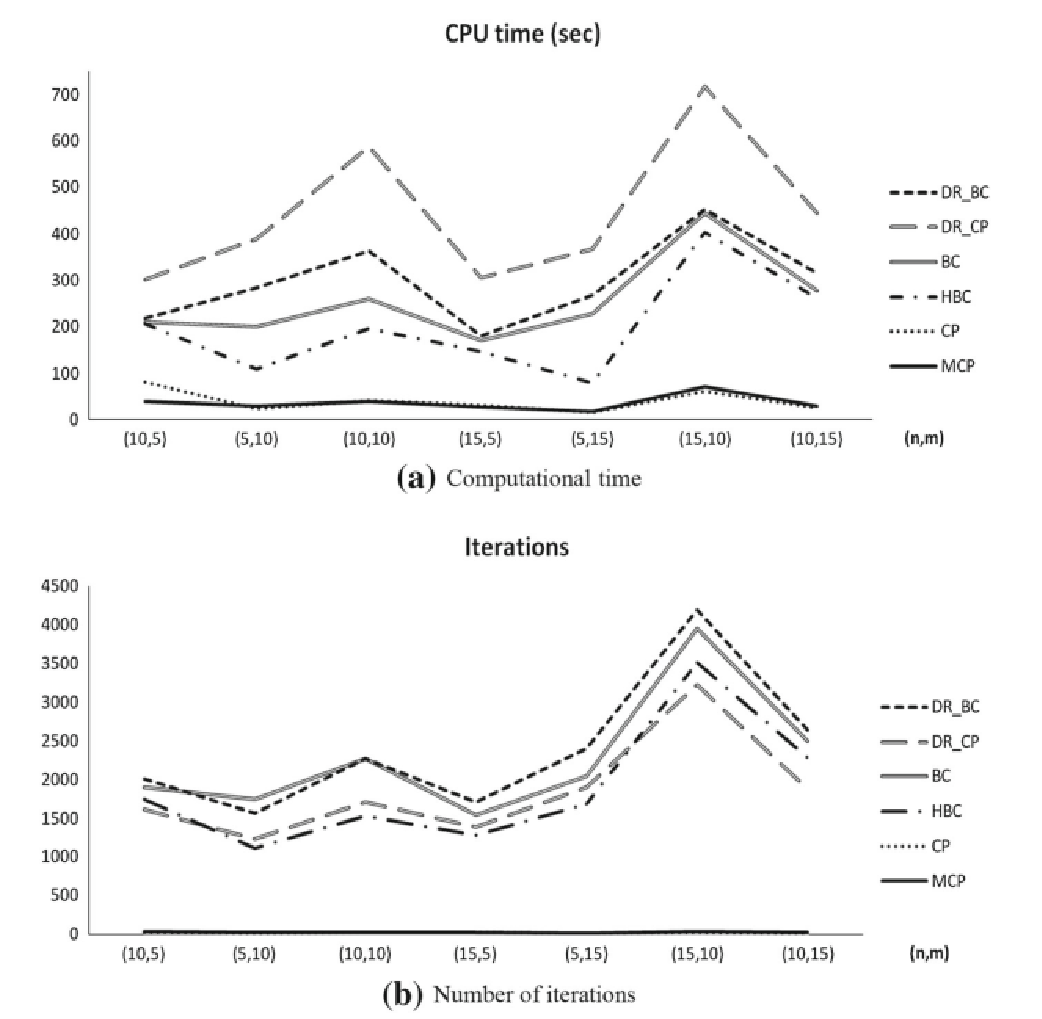
\includegraphics[width = 0.4\textheight]{run-times_2.pdf}
	\caption{Computational comparison for random set}
\end{figure}
\begin{figure}
	\centering
	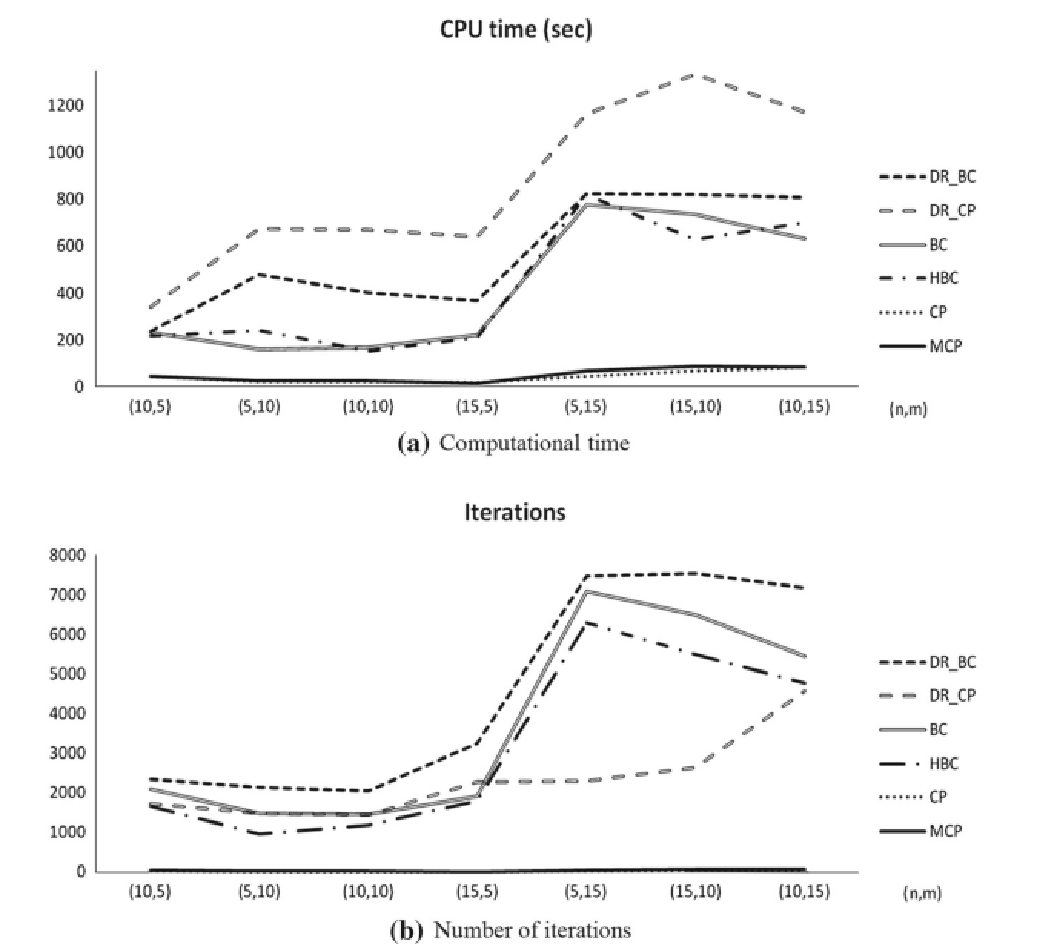
\includegraphics[height = 0.4\textheight]{run-times.pdf}
	\caption{Computational comparison for miplib set}
\end{figure}
	\newpage
	\bibliographystyle{abbrv}
	\bibliography{Bibliography}
\end{document}